\chapter{Desarrollo de servidor web}
\par En este capítulo se describirán los objetivos, el diseño, las prestaciones y la forma en que se llevó a cabo el montaje del servidor web.
\section{Objetivos}
\par Los objetivos de tener un servidor web que disponga de una base de datos y una interfaz visual, como lo es la pagina web son:

    \begin{itemize}
        \item Recabar la información brindada por cada lugar en donde se instale el sistema.
        \item Organizar todos los datos obtenidos en un solo lugar para que cada usuario tenga en forma remota y de fácil acceso las zonas donde se presentan este tipo de hechos. 
        \item Mostrar en forma de tabla cada una de las inhibiciones detectadas.
        \item En base a esta tabla, generar diferentes gráficos que muestren de una forma mas amigable el texto plano.
        \item Tener un lugar de soporte/sugerencias.
        \item Procesamiento matemático para la triangulación y muestra gráfica de la última detección de un lugar de interés. 
    \end{itemize}

\section{Página web}
El dominio es http://www.jammer-detector.ml y la programación de la misma fue realizada en:
\begin{itemize}
    \item HTML, siglas en inglés de HyperText Markup Language, hace referencia al lenguaje de marcado para la elaboración de páginas web. Es un estándar que 
sirve de referencia del software que conecta con la elaboración de páginas web en sus diferentes versiones, define una estructura básica y un código para la 
definición de contenido de una página web, como texto, imágenes, vídeos, scripts, entre otros. Es el estándar que se ha impuesto en la visualización de páginas 
web y es el que todos los navegadores actuales han adoptado.
    \par El lenguaje HTML basa su filosofía de desarrollo en la diferenciación. Para añadir un elemento externo a la página (imagen, vídeo, script, entre otros.), 
este no se incrusta directamente en el código de la página, sino que se hace una referencia a la ubicación de dicho elemento mediante texto. De este modo, la página 
web contiene solamente texto mientras que recae en el navegador web (interpretador del código) la tarea de unir todos los elementos y visualizar la página final. 
Al ser un estándar, busca ser un lenguaje que permita que cualquier página web escrita en una determinada versión, pueda ser interpretada de la misma forma (estándar)
 por cualquier navegador web actualizado.
    \par Es un lenguaje de marcado que nos permite indicar la estructura de nuestro documento mediante etiquetas. Este lenguaje nos ofrece una gran adaptabilidad, 
una estructuración lógica y es fácil de interpretar tanto por humanos como por máquinas.

    \item \par CSS (siglas en inglés de Cascading Style Sheets), en español "Hojas de estilo en cascada", es un lenguaje de diseño gráfico para definir y crear la 
presentación de un documento estructurado escrito en un lenguaje de marcado. Es muy usado para establecer el diseño visual de los documentos web, e interfaces de 
usuario escritas en HTML o XHTML. Junto con HTML y JavaScript, CSS es una tecnología usada por muchos sitios web para crear páginas visualmente atractivas, 
interfaces de usuario para aplicaciones web y GUIs para muchas aplicaciones móviles.

    \par CSS está diseñado principalmente para marcar la separación del contenido del documento y la forma de presentación de este, características tales como las 
capas o layouts, los colores y las fuentes. Esta separación busca mejorar la accesibilidad del documento, proveer más flexibilidad y control en la especificación 
de características presentacionales, permitir que varios documentos HTML compartan un mismo estilo usando una sola hoja de estilos separada en un archivo .css, y 
reducir la complejidad y la repetición de código en la estructura del documento.

    \item \par PHP es un lenguaje de programación de uso general que se adapta especialmente al desarrollo de aplicaciones web dinámicas con acceso a información 
almacenada en una base de datos. El código fuente escrito en PHP es invisible al navegador web y al cliente, ya que es el servidor el que se encarga de ejecutar 
el código y enviar su resultado HTML al navegador.
    \par Es libre, por lo que se presenta como una alternativa de fácil acceso para todos y además posee una amplia documentación en su sitio web oficial, 
entre la cual se destaca que todas las funciones del sistema están explicadas y ejemplificadas en un único archivo de ayuda.
    
    \item \par JavaScript (abreviado comúnmente JS) es un lenguaje de programación interpretado. Se define como orientado a objetos, basado en prototipos, 
imperativo, débilmente tipado y dinámico.
    \par Se utiliza principalmente del lado del cliente, implementado como parte de un navegador web permitiendo mejoras en la interfaz de usuario y páginas 
web dinámicas. 
    \par JavaScript se diseñó con una sintaxis similar a C, aunque adopta nombres y convenciones del lenguaje de programación Java. 
    \par Puntualmente la aplicación que se le dio en este proyecto es realizar operaciones matemáticas para la triangulación y únicamente en el marco de 
la aplicación cliente, sin acceso a funciones del servidor generar gráficas a partir de base de datos, previamente obtenidas mediante el lenguaje PHP. 
\end{itemize}

\subsection{Pestañas}
\subsubsection{Inicio}
Apenas ingresamos a la página podemos observar en la parte superior el logo y nombre del proyecto, y sobre la misma barra en la parte derecha, vemos el menú.
\par En esta pestaña de inicio se coloco la tabla donde muestra la información recabada de todos los lugares donde está instalado el sistema y se encontró 
una inhibición. La información que posee la misma es: ubicación, ID de cada nodo, fecha y hora y el nivel de RSSI y tipo de inhibición detectada por cada uno
 de los nodos. En la figura \ref{web_inicio} podemos ver la misma. 
\begin{figure}[h!]
	\centering
	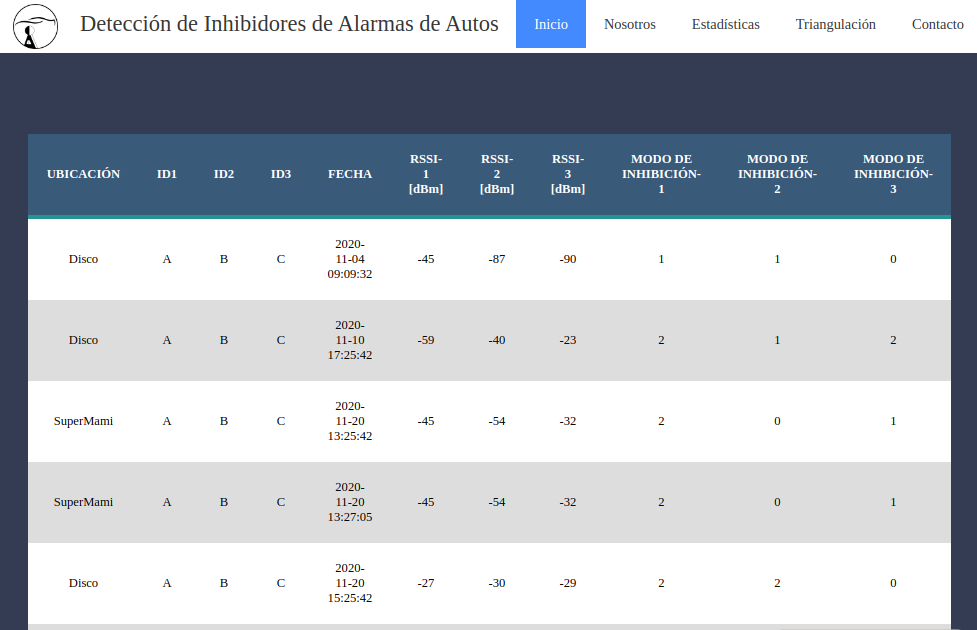
\includegraphics[scale=0.32]{images/web/tabla-web.png}
    \caption{Página de inicio}
	\label{web_inicio}
\end{figure}
\subsubsection{Nosotros}
Esta pestaña está realizada para mostrar la tarjeta de cada uno de los integrantes del grupo de trabajo, dando así también un medio de contacto.
\par En la figura \ref{web_inicio} podemos ver la pestaña. 
\begin{figure}[h!]
	\centering
	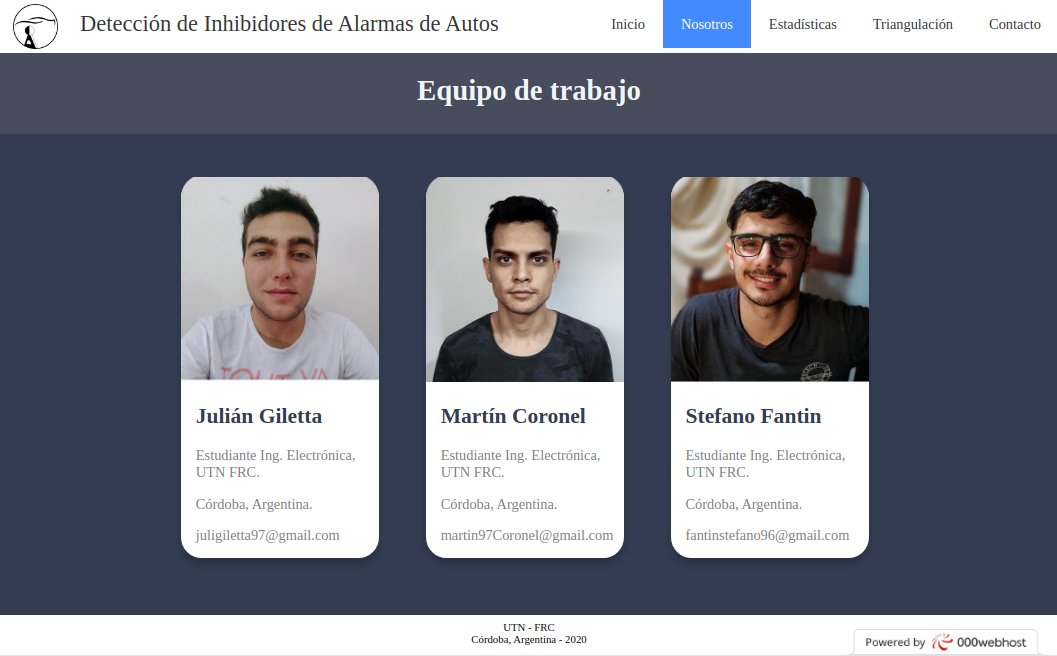
\includegraphics[scale=0.3]{images/web/nosotros-web.png}
    \caption{Presentación de grupo de trabajo}
	\label{web_nos}
\end{figure}
\subsubsection{Estadísticas}
La sección de estadísticas, quizás la mas importante para los usuarios del sistema, es en donde, de una forma gráfica y amigable, se visualizan todos los 
datos representados por los gráficos que mas describan la situación. 
\par En la figura \ref{web_est}, a la izquierda podemos ver un gráfico de torta con las formas de inhibiciones detectadas y a la derecha vemos un gráfico 
de barras que indica la cantidad de inhibiciones por cada lugar. 
\begin{figure}[h!]
	\centering
	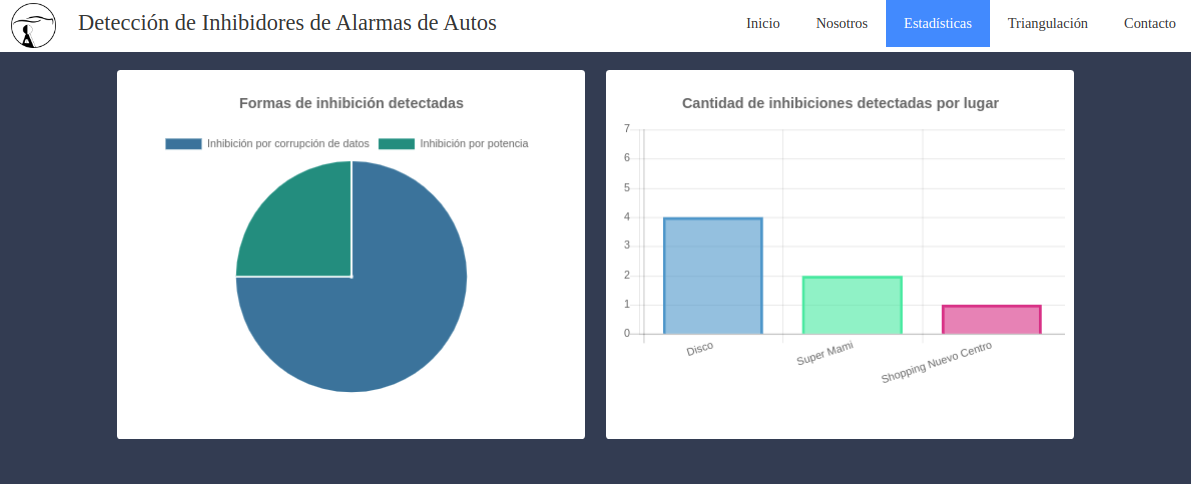
\includegraphics[scale=0.3]{images/web/est-web.png}
    \caption{Gráficos de estadísticas}
	\label{web_est}
\end{figure}
\subsubsection{Triangulación}
\par Esta sección está dedicada al procesamiento matemático y muestra de la triangulación de inhibiciones detectadas por corrupción de
 datos con baja potencia. En la figura \ref{web_triangulacion} un circulo de un radio de 7 metros el cual nos indica la posición de la inhibición detectada.
\par El proceso matemático para el calculo de este punto se basa en la relación de potencia recibida y transmitida de una onda en el espacio libre, considerado 
así para la simplificación de cálculos,  ecuación \ref{eq:rel_potencias}.
 
 \begin{equation}\label{eq:rel_potencias}
    \frac{P_R}{P_T} = \left[\frac{4*\pi*d_1}{\lambda}\right]^{2}
\end{equation}

Operando con la ecuación \ref{eq:rel_potencias} para una misma señal recibida por dos nodos a la vez y haciendo la relación entre ellas obtenemos:

 \begin{equation}
    \left(\frac{d_1}{d_2}\right)^{2} = 10^{\frac{P_dBm_2 - P_dBm_1}{10}}
\end{equation}

 \begin{equation}\label{eq:triangulacion}
    \frac{d_1}{d_2} = 10^{\frac{P_dBm_2 - P_dBm_1}{20}}
\end{equation}

\par Esta relación de distancias nos establece un punto en la recta que une cada nodo entre si (estos se encuentran en los vértices del triangulo azul como se 
ve en la figura \ref{web_triangulacion}), del cual trazando una linea perpendicular a ella, tenemos la linea de acción del inhibidor.
\par Haciendo esta relación entre todos los nodos tenemos 3 lineas que conforman un triangulo por la intersección entre ellas, donde luego obtiene la 
intersección de dos de las mediatrices de estas rectas que nos determinan el centro de la circunferencia que une los 3 puntos encontrados. El punto central, 
con un radio de 8 metros es el área donde se encuentra la inhibición detectada. 


\begin{figure}[h!]
	\centering
	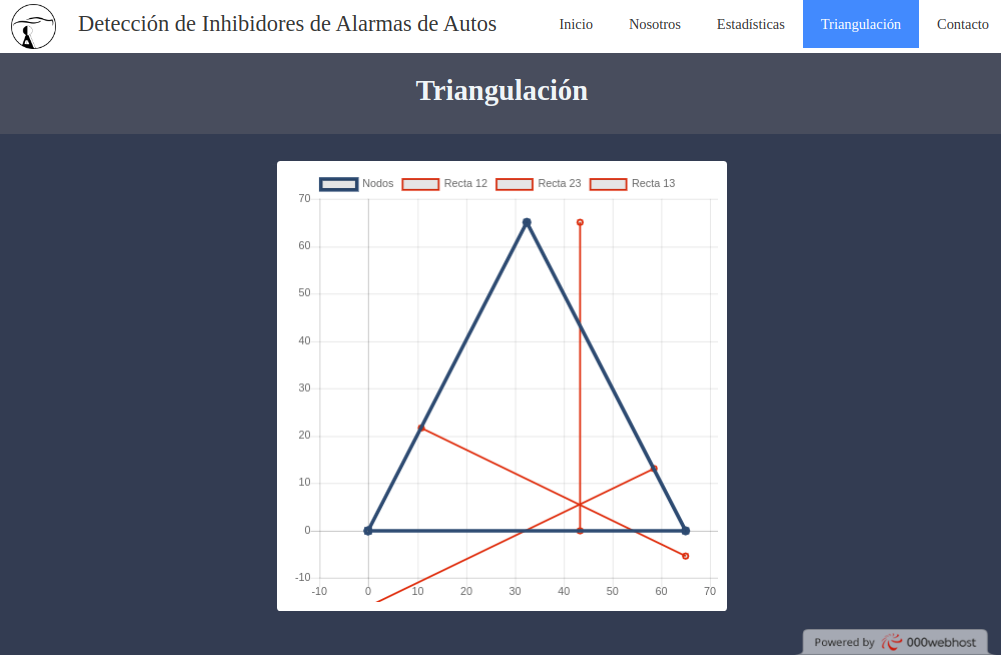
\includegraphics[scale=0.45]{images/web/triangulacion-web.png}
    \caption{Pestaña de triangulación}
	\label{web_triangulacion}
\end{figure}
\subsubsection{Contacto}
Finalmente la ultima pestaña es la de contacto, la cual tiene el fin de que cualquier persona que entre a la página y tenga alguna duda o sugerencia, 
pueda tener un contacto rápido con cada uno de nosotros (figura \ref{web_contacto}).
\begin{figure}[h!]
	\centering
	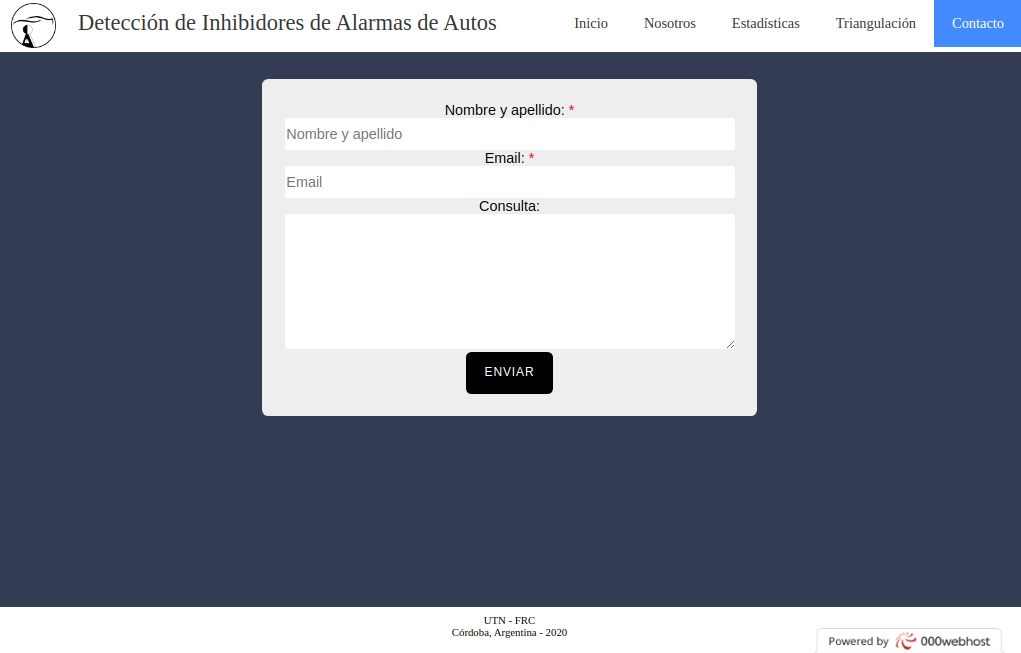
\includegraphics[scale=0.33]{images/web/contacto-web.png}
    \caption{Formulario de contacto}
	\label{web_contacto}
\end{figure}
\section{Base de datos}
La base de datos esta realizada y gestionada en phpMySQL y cuenta con una tabla con el mismo contenido que la que podemos ver en la figura \ref{web_inicio}. \par 
Es el lugar en el cual se almacena cada inhibición detectada y luego, mediante un enlace con la página web, todo su 
contenido es visualizado en esta la misma. 
\subsection{Carga de datos}
\par El enlace desde el servidor web con la central instalada en cada lugar se realiza mediante el acceso a una pestaña oculta de la web, en la cual se interactúa
 con la central mediante un algoritmo de http-POST-request para cargar cada uno de los datos de los nodos correspondientes a cada lugar, para luego procesarlos y 
obtener los gráficos ya mencionados, la triangulación en caso de ser posible y otras utilidades que se le puedan dar. 
